\documentclass[12pt,letterpaper]{article}

%Packages
\usepackage{pdflscape}
\usepackage{fixltx2e}
\usepackage{textcomp}
\usepackage{fullpage}
\usepackage{float}
\usepackage{latexsym}
\usepackage{url}
\usepackage{epsfig}
\usepackage{graphicx}
\usepackage{amssymb}
\usepackage{amsmath}
\usepackage{bm}
\usepackage{array}
\usepackage[version=3]{mhchem}
\usepackage{ifthen}
\usepackage{caption}
\usepackage{hyperref}
\usepackage{amsthm}
\usepackage{amstext}
\usepackage{enumerate}
\usepackage[osf]{mathpazo}
\usepackage{dcolumn}
\usepackage{lineno}
\usepackage{color}
\usepackage[usenames,dvipsnames]{xcolor}
\pagenumbering{arabic}

%Pagination style and stuff
\linespread{2}
\raggedright
\setlength{\parindent}{0.5in}
\setcounter{secnumdepth}{0} 
\renewcommand{\section}[1]{%
\bigskip
\begin{center}
\begin{Large}
\normalfont\scshape #1
\medskip
\end{Large}
\end{center}}
\renewcommand{\subsection}[1]{%
\bigskip
\begin{center}
\begin{large}
\normalfont\itshape #1
\end{large}
\end{center}}
\renewcommand{\subsubsection}[1]{%
\vspace{2ex}
\noindent
\textit{#1.}---}
\renewcommand{\tableofcontents}{}

\begin{document}


Dear Dr D\'{a}valos,

MPE-15-254: Interim Decision

We are very grateful to both referees for their helpful and constructive comments, which we believe have helped us to significantly improve our paper. We have taken all of their comments on board, and respond to their points below. For improving clarity in this document, we sorted the reviewers comments as follows:
\begin{enumerate}
\item \textbf{Reviewer 1:} containing reviewer's 1 major comments
\item \textbf{Reviewer 1 Specific comments:} containing reviewer's 1 specific comments
\item \textbf{Reviewer 2:} containing reviewer's 2 comments
\end{enumerate}
Also, we uploaded two versions of the revised manuscript. Both have the exact same content but one has all the changes and additions to the main text highlighted in yellow.

% TG: actually, is it possible to send them the response as a pdf or will I have to copy paste all that in a mail? If the second, it's not that a big problem (just annoying) but I think we should try sending the pdf, it's way clearer like that.


\section{Reviewer 1:}

\begin{enumerate}
\item{\textcolor{blue}{\textbf{Novelty:} The novelty of this study should be spelled out more clearly by more a more thorough review of the literature, not just by referring to a few relevant works, but by pointing out what is so new about this study.
The authors assert that this is the first study to examine the effects of missing morphological data from a total evidence dataset, but that is what Pattinson et al. 2014 did (as well as Wiens 2005).
This study examines it in a different way with a study design that is unique and adds to the field. For example, one feature of this study that is unique is that a tree with fossils is simulated and the data simulated on that tree.
In other studies of missing data, data were removed from living taxa to determine if their positions could still be inferred (Pattinson et al. 2015; Wiens and Tiu 2012).
This study will have bearing on an old assertion that including fossils specifically may help alleviate long-branch attraction, not only additional taxa with varying amounts of missing data, as suggested by others (e.g., Wiens 2005).
Similarly, in the discussion, the authors need to point out how their results fit in with the results of previous research more clearly. }}

% The novelty of this study should be spelled out more clearly by more a more thorough review of the literature, not just by referring to a few relevant works, but by pointing out what is so new about this study.

% The authors assert that this is the first study to examine the effects of missing morphological data from a total evidence dataset, but that is what Pattinson et al. 2014 did (as well as Wiens 2005).

% This study will have bearing on an old assertion that including fossils specifically may help alleviate long-branch attraction, not only additional taxa with varying amounts of missing data, as suggested by others (e.g., Wiens 2005).

% Similarly, in the discussion, the authors need to point out how their results fit in with the results of previous research more clearly.




\item{\textcolor{blue}{\textbf{Graphical abstract:} Current graphical abstract does not capture the content of the article for readers in a single glance.
The authors should not use red and green together.
Figure 5 illustrates topology distance with different inference methods and varying proportions of missing data in rows vs columns and would make a better graphical abstract.
For the graphical abstract, Fig 5 needs to be made clearer in one glance what is going on.
More details are given in the comments on that figure below.}}

We gladly followed reviewer 1's graphical abstract suggestions and have changed it to be similar to the figure 5. % TG: It's freaking not catchy at all but at this point I give up. I've tried many ways but the flippin' paper IS NOT attractive. It might be useful, well written, interesting, citable, etc... But it won't be sexy.



\item{\textcolor{blue}{\textbf{Highlights:} wording seems awkward}}

We rephrased the highlights of the paper as follows: %3 to 5 bullet points (maximum 85 characters, including spaces, per bullet point). TG: probably need improvement here.

\begin{enumerate}[(1)]
\item The Total Evidence methods allows to combine living and fossil data.
\item This study test the effect of missing morphological data on topology.
\item The number of living taxa with data as the most effect on recovering topology.
\item Bayesian inference outperforms Maximum Likelihood for correct clade recovery.
\item We suggest that the sampling effort should be focused on data for living taxa.
\end{enumerate}



\item{\textcolor{blue}{\textbf{Introduction:} Needs stronger emphasis on what specifically is unique about this study compared to what the many other studies on missing data have done and found.
Clearly outlining the questions in this study that are left open from previous research is important because some of the findings in this study suggest that there may be more error associated with missing data than previous research has suggested.}}

% Needs stronger emphasis on what specifically is unique about this study compared to what the many other studies on missing data have done and found.
% To do (see reviewer 1 specific comment 13) - links to major comment one on novelty

% Clearly outlining the questions in this study that are left open from previous research is important because some of the findings in this study suggest that there may be more error associated with missing data than previous research has suggested.



\item{\textcolor{blue}{\textbf{Abbreviation:} One suggestion is to consider abbreviating Maximum Likelihood and Bayesian Inference as ML and BI respectively early in the methods and use throughout.}}

We do understand the reviewers concern are agree that ML and BI are two commonly used abbreviations.
Nonetheless, we would rather prefer not abbreviate these terms: in fact, even though they might add some concision to the sentences where Maximum Likelihood and/or Bayesian Inference are stated, we think they might add confusion or difficulties to the whole paper.
Spelling out the abbreviation might be locally less concise (i.e. in the sentence) but at least are completely clear and does not ask the reader to look back for the actual meaning of such or such abbreviation (Berlin 2013; Radiology; \url{http://pubs.rsna.org/doi/abs/10.1148/radiol.12121776}).
However, we leave this decision to the editor if she judges it better to abbreviate those terms. % TG: or maybe this statement is useless? Of course we leave it to the editor...



\item{\textcolor{blue}{\textbf{Methodology - True tree:} I suggest it warrants comparing at least the 'best' tree to the 'true' tree.}}

We compared both the ``best'' tree and the ``missing-data'' trees to the ``true'' tree as suggested by both reviewer.
We did not, however, include the results to the main text (available in appendix B; figure B1 and appendix C; figures C6 and C7).
We do agree with the point raised with both reviewers on comparing the true tree to the best/missing-data trees.
As reviewer 1 states: "[this analysis can give] insights to whether the parameter settings used in the simulations and in the analyses were adequate for generating datasets and inferring the true tree, or something close to it.".
However, even though we agree with the comments of both reviewer that knowing the difference between the true and best/missing-data trees is important, we do not think that it "adds an additional layer of complexity that can't be accounted for via simulation" (reviewer 2, comment 1).
In this simulations, we had to make a choice between (1) simulating larger matrices but with less chains (i.e. less variance) or (2) smaller matrices with more variance.
We deliberately made the second choice because our main question was "what is the effect of our parameters on recovering the topology".
In fact, regarding our problematic, we maintain that comparing the best tree to the missing-data trees is the best approach to answer this specific question for two reasons:
\begin{enumerate}
\item{The true tree is always unknown:} as we state in the manuscript: "In real world situations, the ``true'' tree is never available" (line 242 in the first manuscript and @@@ in the revision).
\item{The true tree is just the starting point of the simulations:} in fact, we use the true tree only as a starting point for our simulations. Once generated, the true tree is fed to a cascade of algorithms and softwares (i.e. seqGen\{phyclust\}, rTraitDisc\{ape\}, RAxML, MrBayes) described in section 2.1 and 2.3 in order to get the best tree and the missing-data trees. Comparing the latests to the true tree will answer to the problematic "what is the effect of our missing-data parameters and the cascade of algorithms and softwares on recovering the true topology?".
\end{enumerate}
Therefore we added the second justification to the main text (see below this response) and added these analysis (true vs. best/missing-data trees) to the supplementary for potential readers that might be interested by this specific problematic.

We added the following sentence to the main text to clarify and link to the supplementary analysis:
"In practice, the difference between the ``true'' and the ``best'' tree represents the effect of our parameters and R packages choices (i.e. diversitree, phyclust and ape) as well as the phylogenetic methods used (see appendix B).
The aim of this study, however, is to look at the effect the missing data parameters described above on topological recovery." (line @@@).



\item{\textcolor{blue}{\textbf{Methodology - Starting tree:} The authors should at least include some analysis in which no starting tree is given, the max. likelihood 'best' tree is given, and / or the 'best' tree is given but with some perturbation.
I fear that one of the main results may be biased due to this one methodological detail - a strong prior on tree topology.
The justification given was 'to speed up the Bayesian analysis' which does not seem adequate, given these datasets are small.}}

We dealt with this legitimate suggestion an extra analysis on a subset of five trees with the three missing data parameters at 0\%, 10\%, 25\%, 50\% and 75\% for 20 chains. 
We compared the topology of these trees in Bayesian inference when using the true tree as a starting tree or using a random tree (default in MrBayes) as a starting tree.
We found no difference in topologies between both the Bayesian inferences starting with the true tree or a random tree.
We made these data available in the supplementary materials Appendix A (figure A2 and tables A1 and A2) and we also added a precision in the manuscript:

"We used a fixed starting tree rather than a random starting tree (default MrBayes; Ronquist et al., 2012b) to speed up our Bayesian inferences.
Note that a starting is not a Bayesian prior on topology \textit{per se} and did not significantly affected topology (see Appendix A, section ``Effect of the starting tree on Bayesian inference'')." line @@@ 



\item{\textcolor{blue}{\textbf{Results - Bhattacharyya meaning:} Some descriptive statistics are given, but it would help to tell us if these differences are meaningful.
For example, on line 414 the Bhattacharrya Coefficients are given suggesting RF distances are lower for ML than BI trees at 0.69, 0.48, and 0.66 - but if this coefficient represents the probability of overlap between distributions then shouldn't the coefficients be $<$0.05 to say that one is lower than the other?
In the table, mean and median values of $<$0.01 and $>$0.85 are highlighted as being the most extreme.
Later the focus on Bhattacharyya Coefficients is 1 when distributions overlap completely and 0 when they do not - should this be the criterion?
Just make it clear early on so the readers knows what to think when they see these numbers. }}

We clarified the interpretation of the Bhattacharyya Coefficient throughout the manuscript.
We advocate that two distributions are significantly different when their probability of overlapping (the Bhattacharyya Coefficient) is $>$0.05 and that they are significantly similar when this probability is $>$0.95.
Even though other values (e.g. 0.85) are not conclusive, we still reported them to show the relative overlap of the distributions (i.e. two distributions with a coefficient of 0.85 are not significantly similar but are closer to each other than two distributions with a coefficient of 0.15; which are themselves not significantly different but still less closer to each other than the previous ones).
We added the following statement to the main text and to the appendix B:

"When the Bhattacharyya Coefficient between two distributions is $<$0.05, the distributions are significantly different.
When this coefficient is $>$0.95 both distributions are significantly similar.
Values in between these two threshold just show the probability of overlap between the distributions but are not conclusive to assess the similarity or differences between the distributions." line (@@@)



\item{\textcolor{blue}{\textbf{Results - Bayesian consensus vs. Bayesian posterior:} One major finding that was not fully addressed was that the distances between the BI posterior distributions of trees do not overlap the BI best or consensus trees.
It seems from the tables in Appendix C that the topology distance metrics for Bayesian posterior distribution are similar to those for the Bayesian consensus, albeit usually lower for RF distance than the Tr distance.
In Figure 4, it seems like the distributions of metrics based on CIs for Bayesian consensus and posterior overlap up until >25\% missing data.
How then in comparisons of the distributions are they always so low (Table 1 max prob. of overlapping distributions = 0.11)?}}

The difference between the Bayesian consensus and the Bayesian posterior trees can be due to two factors:
\begin{enumerate}
\item first, the way we assess topological recovery is slightly different in each case: for the Bayesian consensus trees, we simply compared the "missing-data" consensus tree to the "best" consensus tree; for the Bayesian posterior trees however, we randomly compared 1000 "missing-data" Bayesian posterior trees to 1000 "best" Bayesian posterior trees.
Therefore, even if the comparison methodology is the same, the fact that the second methods draws random trees, we expect the topological recovery score to be "blurred" in comparison to other comparisons that do not involve random comparisons.
\item secondly, the Bayesian posterior trees are always resolved and thus, in the same way as the Maximum Likelihood tree, more likely to contain "false-positive" nodes. On the other hand, because the consensus tree is a strict majority consensus rule, only nodes with a a good support will be represented in the tree and all other nodes will be collapsed. This reduces the amount of "false-positive" nodes (since an unresolved tree is always better than a wrongly resolved one) and increases clade conservation but also increases the placement of wild-card taxa (since it is likely that some Triplets will just not exist in a poorly resolved consensus tree).
\end{enumerate}
Both points were discussed in the former manuscript lines 566 and 573 (or lines @@@ and @@@ in the revised version).
We expanded the paragraph to:

"Additionally, the Bayesian posterior trees performed way worth than the Bayesian consensus tree (figure 4, table 1 and appendix C figure C5 and tables C5, C6 and C7).
This can be due to the fact that the Bayesian posterior trees are always resolved and thus more likely to contain wrongly resolved nodes (i.e. decreasing the Normalised Robinson-Foulds metric).
Conversely, the Bayesian consensus tree might not resolve nodes that are badly supported and thus more likely to contain only correctly resolved nodes (i.e. increasing the Normalised Robinson-Foulds metric)." lines (@@@)

Concerning the last question of this comment: "How then in comparisons of the distributions are they always so low (Table 1 max prob. of overlapping distributions = 0.11)?" when looking at all parameters separately (figure 4), there is no clear overlap between the Bayesian consensus trees and the Bayesian posterior trees (median Bhattacharyya Coefficient of 0.01; table 1).
The maximum observed Bhattacharyya Coefficient (0.11; table 1) is probably due to the combination of parameters: when all the parameters have many missing data, the probability of overlap between trees was slightly higher (0.11) but still really low.
For the Normalised Triplets distance however, the overlap is higher (median Bhattacharyya Coefficient of 0.59; table 1) as illustrated in figure 4 (i.e. much more overlap between the distributions).

% TG: I'm confused for the second part of the question:
% TG: In figure 4 and in Table 1, if you look at the Bayesian consensus (grey) trees and the Bayesian posterior trees (orange) for RF, they do not really overlap. Ever. The 0.11 probability must come from the parameters combinations that, when is really shitty must show a little bit of overlap. But for each parameter one by one: nope. No overlap.
% TG: On the other side, in figure 4 and Table 1, for Bayesian consensus and Bayesian posterior for Tr, the do overlap much more. And that's what's in the Table 1 (min 0.21; median 0.56; and max 0.87).
% TG: Did the reviewer just miss read the labels of the Table 1 or am I miles away from what he means?




\item{\textcolor{blue}{\textbf{Results - Bayesian Triplets:} Another important result that is not mentioned is that using the wildcard taxon metric (Tr), Bayesian consensus trees do quite poorly with missing data.
Values in Figures 4 and 5 clearly drop below zero, although negative values are not illustrated on the axis, and this indicates that the tree topologies are no better than, or even worse than, random trees.
It is especially true when fossils are missing data, and that is going to be an important finding with practical application but must be addressed. }}

We modified the figures 4 and 5 to show Normalised Triplets metric values below 0 and added a dashed line at 0 to underline the difference in scale between both metrics.
As mentioned above (reviewer 1 comment 9), this is due to the fact that the Bayesian consensus tree will be less and less resolved when missing data increases.
This has two related effects.
The first one being to retain "good" clade conservation (i.e. avoiding "false-positive" nodes by collapsing unsupported ones).
And the second one is that when these clades are collapsed, it reduces the amount of available triplets and thus increases the "wild-card taxa" score (Normalised Triplets metric).
In fact, when a clade ((a;b);c); is collapsed to (a;b;c), the whole clade is conserved (a, b and c are still in a common clade) however they also all become wild-card taxa: the position of a regarding b and c is now incorrect.

We added a precision on this point in the...
% TG: add a paragraph in the results about the wild-card fossils

% TG: STOPPED HERE.




\item{\textcolor{blue}{\textbf{Conclusion:} The authors should clarify how their results compare to those of previous studies more directly to emphasize the nuances that make this study unique. }}

We modified the conclusion as follows (see reviewer 1 specific comments 52)



\item{\textcolor{blue}{\textbf{Figure 4:} Figure 4 has a color scheme issue, the colors in the caption do not match up to the figure.}}

We apologies for this silly mistake and fixed the colors in the figure. We also changed the color scheme to match with the general color scheme of the paper (black, grey, orange and blue).



\item{\textcolor{blue}{\textbf{Figure 4-5:} Am I wrong or shouldn't the y-axis for Normalised Triplets metric go below 0 - it looks those metrics for many missing data combinations have values below zero indicating trees are more different from the 'best' tree than expected by chance (Appendix B 1.1., see Appendix C Tables 1-3) and that is important to show.}}

We fixed this graphical mistake as state above in reviewer 1 specific comment 13.



\item{\textcolor{blue}{\textbf{Table caption:} Table caption should include a line about 'pooling across missing data schemes' to clarify what is presented.}}



\item{\textcolor{blue}{\textbf{Previous research:} The missing-data problem has a long history in the literature and there are references to some of those older and recent papers.
But I feel it is necessary to summarize the following questions: what did those studies find, what are the questions those studies left open, and how does this study address them?}}

% specifically state line by line where we dealt with which and which question.

\end{enumerate}

\section{Reviewer 1 Specific comments:}
\begin{enumerate}

\item{\textcolor{blue}{\textbf{line 31:} has it really been shown that the majority of macroevolutionary studies focuses on extant species only? The cited references are examples of large scale extant-only phylogenies. To make such a pointed statement, the authors would need to find support from some kind of literature review or meta-analysis comparing the number of paleontological to neontological macroevolutionary studies. Otherwise, rephrase. }}

We revised this statement as follow: "many large-scale macroevolutionary studies focus solely on living species" (line @@@).

\item{\textcolor{blue}{\textbf{line 37 and throughout:} Rephrase so that 'however' does not start the sentence, such as 'To do this, however, we need…'. Sentences should not start with however if the meaning is to contrast with the previous statement (Strunk, W. and White, E.B. 2009. The Elements of Style. NY: Pearson Education. p 48-49).}}

We thank the reviewer for this stylistic suggestion and modified the placement of 'however' throughout the manuscript.

\item{\textcolor{blue}{\textbf{line 43:} sentence choppy, consider rephrasing or splitting into two sentences.}}

We modified the sentence as follow: "These approaches differ mainly in how they treat the fossil taxa and it's data. One can use the fossil as tips or as nodes in the phylogeny and use it's age only, it's morphology only or it's age and morphology jointly." (line @@@)

\item{\textcolor{blue}{\textbf{line 44:} three alternatives: age only, morph only, or age and morph jointly. }}

See previous change (Specific comment number 3).

\item{\textcolor{blue}{\textbf{line 47:} Simpson 1944 doesn't seem the appropriate reference for maximum parsimony. Consider (Felsenstein 2004; Hennig 1966) }}

We modified the citation as suggested by reviewer 1 (line @@@).

\item{\textcolor{blue}{\textbf{line 53:} omit 'are used as nodes rather than tips in these phylogenies and their'. Fossils aren't really used as nodes in node calibration, the second part of the sentence is more accurate.}}

We modified the following sentence as suggested: "Because fossil taxa do not usually have available DNA, only fossils' occurrence dates are used to time calibrate phylogenies" (line @@@).

\item{\textcolor{blue}{\textbf{line 66:} omit 'have been successfully applied to empirical data' and just say 'becoming increasingly popular…list of references'. }}

We modified the following sentence as suggested: "Total Evidence methods is becoming an increasingly popular way of adding fossil taxa to phylogenies (e.g. ...)" (line @@@).

\item{\textcolor{blue}{\textbf{line 76 and throughout the manuscript:} watch out for inconsistent parentheses.}}

We fixed this issue.

\item{\textcolor{blue}{\textbf{line 76 and throughout:} correct use of the word 'data' from singular to plural throughout}}

% TG: actually I'm not going to change it:
We thank the reviewer for pointing out this inconsistency, however, 'data' is now commonly used for the singular case (Pinker, S. \textit{The Sense of Style: The Thinking Person's Guide to Writing in the 21st Century}. Penguin, 2014. p 271; and Guardian and Observer style guide (2015): \url{http://goo.gl/cmKjNe}).

\item{\textcolor{blue}{\textbf{line 77:} change 'a lot' to 'large proportions of' or something more accurate and less colloquial}}

We modified the following sentence as suggested: "Total Evidence matrices are likely to contain a large proportions of missing data" (line @@@).

\item{\textcolor{blue}{\textbf{line 82:} change to '…missing data are not phylogenetically biased, Wiens…'}}

We modified the following sentence as suggested: "as long as enough data overlaps in each case, and missing data are not phylogenetically biased" (line @@@).

\item{\textcolor{blue}{\textbf{line 99:} unclear - what is meant by 'with a fixed topology approach'? The studies references investigated divergence times using total evidence datasets and in some cases used constraints but not completely fixed topologies}}

We modified the previous statement to: "but also because previous studies have already empirically assessed the effect of the Total Evidence method on branch length variation but using topological constraints" (line @@@).

\item{\textcolor{blue}{\textbf{lines 80-103:} (1) the authors need to clearly justify the importance of this study compared the many studies that have investigated the effects of missing data on topology inference.
The justification currently given is not particularly strong and the specific unique questions asked in this study that are currently unanswered should be made clear.
The current argument does not always seem justified by the literature review.
For example, line 81 the authors argue that papers by Wiens and Pattinson examined morphological or molecular matrices separately, but in Pattinson, for example, combined datasets for living species were used to simulate extinct species by deleting the molecular and parts of the morphological datasets from living species.
The authors could argue that a limitation of the Pattinson study, which they address here, was the limited scheme for generating missing data from the datasets.
In this study, the authors perturbed the datasets more thoroughly in a clearly structured experimental design to investigate the effects of eliminating living versus fossil data or all data overall.
That is one aspect of this study that I perceived as new and unique.
(2) Another aspect of this study design that could be new but is not explored here is the effect of the missing data on the morphological substitution rate parameter estimates.
Can you recover the true values from the perturbed datasets?
This study also used a unique way of evaluating the tree inference under missing data scenarios.
These and other aspects of the study uniqueness must be clearer.}}

(1) - We thank the reviewer for this judicious comment and emphasized on both the novelty aspect of our study and on the questions we are actually testing as follow:

"Until now, only few attempts have been made to study study the impact of this missing data issue on phylogenetic inference in a Total Evidence framework (i.e. using combined molecular and morphological data; e.g. Wiens et al., 2005; Pattinson et al., 2014). For example, Wiens et al. (2005) only assess the effect of missing data by comparing the node support between the complete dataset that contains missing data and sub-datasets with no missing data. Furthermore, Pattinson et al. (2014) assess the effect of removing both molecular and morphological data (“artificial extinction”) on the topology. These studies, however, are limited by their empirical-only approach (Wiens et al., 2005) and the scheme of generating missing data (Pattinson et al., 2014)."

"In this study, we propose a theoretical assessment of the effect of missing data in the Total Evidence method by thoroughly eliminating living or fossil data or all data overall. We test the effect of missing data by measuring two crucial aspects of topology in both Maximum Likelihood and Bayesian Inference methods: (i) the conservation of clades and (ii) the displacement of wild-card taxa."

(2) - the second point underlined by the reviewer in this specific comment strikes use as really interesting. However, we considered this study to be already long and complex. We therefore think that adding an extra question to this study (i.e. what is the effect of missing data on the morphological substitution rate parameter estimates?) might loose the reader.
Nonetheless, we added the result of such analysis in the \textbf{Appendix-A Morphological rates estimations results} section.
We linked to this analysis in the methods part as follows:
"The detailed MrBayes parameters are available in Appendix A along with details on the $\alpha$ parameter estimation."

% TG: what do you think? I don't want to attract the reviewer's attention too much (i.e. that's another shit load of analysis to do to do it properly) and certainly not the reader's attention either (it's not relevant to the whole paper) but sticking that to the supplementary kind of does what the reviewers wants to know.

\item{\textcolor{blue}{\textbf{line 124:} replace 'sections' with 'partition'}}

We modified the following sentence as suggested: "the morphological partition of Total Evidence matrices" (line @@@).

\item{\textcolor{blue}{\textbf{line 125:} omit 'note that we explain each step in detail below this general outline', replace with something like 'Our general protocol included the following steps (Figure 1):'…}}

We removed the part suggested by the reviewer as follow: "we used the following protocol (Figure 1):" (line @@@).

\item{\textcolor{blue}{\textbf{line 167 and throughout manuscript:} replace usage of 'inferred' when referring to simulating data. Replace with 'generated', 'simulated', or 'created', for example. 'Infer' should only be used when a model is fit to data to infer some output such as a tree, transition rates, etc. }}

We replace 'inferred' by 'simulated' on lines @@@ and @@@ %LaTeX lines 192 'The molecular matrix was simulated' and 199 'We simulated the morphological matrix using the R'

\item{\textcolor{blue}{\textbf{line 173:} streamline to "The substitution rates were selected from a gamma distribution with…" or something similar. }}

We modified the following sentence as suggested: "The substitution rates were selected from a gamma distribution with an ($\alpha$) shape of 0.5." (line @@@).

\item{\textcolor{blue}{\textbf{line 173 to 176:} need some justification for why the substitution rate with alpha shape of 0.5  will avoid homoplasy. Yang 1996 is cited but clarify the justification of what is 'too much' homoplasy. }}

We changed the sentence to:
"In practice, such a value of $\alpha$ $<$ 1 decreases the number of sites with high substitution rates, thus reducing homoplasic sites and increasing the phylogenetic signal (Hassanin et al., 1998; Estoup et al., 2002).%\citep{Hassanin1998611,EstoupHomoplasy}.
Also, we chose this low value to be consistent with our protocol for simulating morphological characters (see below)." (line @@@).

\item{\textcolor{blue}{\textbf{Line 176 to 180:} could be streamlined. It is not clear what is meant by 'no special assumption about how the characters evolved', what constitutes a special assumption? Could potentially be reduced to something like 'this model and these parameter settings strike a balance between realism for empirical datasets (citations) and parameter richness with more complex models (e.g., GTR, multiple partitions with independent models), making them more suitable for our computational limitations'. Just for example.}}

We modified the sentence as follows:
"We selected this model and parameters settings to be a compromise between realism from empirical datasets (e.g. Kelly et al., 2014) and models with few parameters (cf. Springer et. al., 2012) to reduce the computational time required if these parameters were estimated rather than defined in the tree building part of the analysis (even with the parameters defined, the total computational time for the whole analysis was around 150 CPU years)."

\item{\textcolor{blue}{\textbf{line 182:} give the ape function used}}

We modified the sentence as follows: "We simulated the morphological matrix using the rTraitDisc function from the R package ape v. 3.0-11 (Paradis et al., 2004) to generate a matrix of 100 character sites for 51 taxa."

\item{\textcolor{blue}{\textbf{line 185 to 188:} streamline, e.g. '…sampling with a probability of 0.85 for two states characters and 0.15 for three state characters (based on an empirical review of published matrices, see Appendix A).'}}

We modified the following sentence as suggested: "sampling with a probability of 0.85 for two states characters and 0.15 for three state characters (based on an empirical review of published matrices, see Appendix A and Fig. A1 within)." (line @@@).

\item{\textcolor{blue}{\textbf{line 193 to 196:} again, justify why gamma with shape of 0.5 is appropriate for minimizing homoplasy. This distribution places highest probability on substation rates less than 0.5, when one of the cited references potentially suggests that the lowest topological error was found at rates of ~0.5-1.5, and that very low substitution rates incurred error similar to very high rates ((Wright and Hillis 2014) 2014 Figure 3). Other cited references do not clearly state that this distribution and shape setting is optimal, so the authors really must justify. }}

We initially chose this parameter from personal communication with April Wright and to be consistent with the molecular rate parameter.
We like to point out that, in figure 3 from Wright and Hillis 2014, even if the Topological error is high when rates are near 0, it is mainly the case for parsimony and both parsimony and Mk with missing data, the fitted model for the Mk model with no missing data (light purple line) is still at lowest when the rates are near 0.
Topological error, however, becomes minimal for all scenari (Parsimony and Mk, with or without missing data) at a rate of 0.5 (see modified figure 3 from Wright and Hillis (2014) in this response; we added the tick marks and the 0.5 rate limit by using the ruler in Adobe Illustrator).

\begin{figure}[]
\centering
    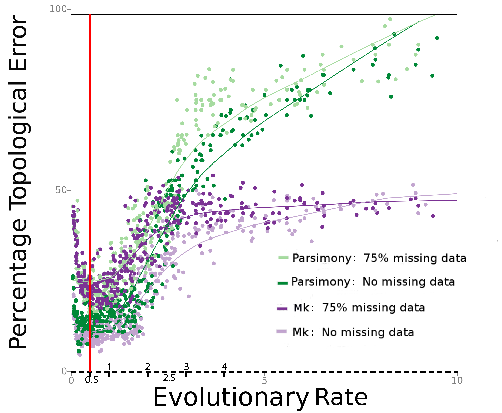
\includegraphics[keepaspectratio=true]{response_fig1.pdf}
\caption{Figure 3 from Wright and Hillis 2014 with added x axis ticks. The red line represents the 0.5 rate.}
\end{figure}

We do agree, however, that if rates get lower than 0.5, variance in topological error increases (especially for the Mk model with missing data).
Therefore, we implemented the \textit{a posteriori} matrix selection step to our analysis (i.e. keeping only the ``complete'' matrices that led to trees with a median bootstrap $>$ 50; explained lines 259-268 in the submitted manuscript and lines @@@ and @@@ in the revised one).

We rephrased the section underlined by the reviewer as follows:

"We used low evolutionary rate parameters to be consistent with the molecular rates parameters and to avoid homoplasy in the morphological part of the matrix and create a clear phylogenetic signal (Wright and Hillis, 2014). Note that Wright and Hillis (2014) have shown that low morphological rates (< 0.5) increases variance in topological error but we discarded simulations with such topological error by selecting only matrices with a “fair” phylogenetic signal (see Estimating phylogenies section below; Zander, 2004)."

\item{\textcolor{blue}{\textbf{line 201:} change 'get' for 'obtain' or something less colloquial.}}

We modified this whole section following reviewer 2 comment 2.

\item{\textcolor{blue}{\textbf{line 231-235:} streamline, e.g., 'The minimal dataset included in this study was 5\% of the morphological matrix for any taxon'.}}

We modified the sentence as follows: "To avoid avoid matrices containing taxa without any data (morphological or molecular), we repeated the random deletion until the matrices contained at least 5\% of data for any taxon." (line @@@).

\item{\textcolor{blue}{\textbf{line 237-246:} I understand the rational presented by the authors for comparing missing data trees to the best tree inferred from max. likelihood/Bayesian techniques rather than compare missing data trees to the true tree used to simulate the data. I still feel it would be an important contribution to this paper, however, to compare the missing data trees to the true tree to evaluate the effects of missing data on the tree inference. Also it may lend insights to whether the parameter settings used in the simulations and in the analyses were adequate for generating datasets and inferring the true tree, or something close to it. }}

We dealt with this comment above (Reviewer 1, major comment 6) and below (Reviewer 2 comment 1).

\item{\textcolor{blue}{\textbf{line 249:} condense citations to one parenthetical statement, 'GTR model (Tavare, 1986, default setting in RAx…)'. Also watch for citations in parentheses inside of other parenthetical statements on line 250 and throughout the manuscript. }}

We fixed these issues throughout the manuscript.

\item{\textcolor{blue}{\textbf{line 251:} omit 'implemented'}}

We removed this word.

\item{\textcolor{blue}{\textbf{line 273:} 'Bayesian Inference'}}

We changed the title as suggested.

\item{\textcolor{blue}{\textbf{line 286:} Why was the true tree used as a starting tree? Earlier the authors argued that the true tree is almost never known, so using it here detracts from the generalizability of these results. If the only justification is 'to speed up the Bayesian estimation process' as stated later, then it seems like this may bias one of the main results, which is that Bayesian analyses outperformed max. likelihood, in which no starting tree was used. I understand the computational limitations, but the authors should present some analysis with complete and missing data in which no starting tree is given compared to analyses in which a starting tree is given to evaluate whether using a starting tree significantly affects the resulting trees, perhaps in an Appendix. Or at least include some perturbation to the starting tree to avoid overly influencing the resulting topology. It would seem to me that this is illustrated in figure 5, where-in with the Robinson-Foulds metric, the distance to the best tree in Bayesian analysis seems to have a lower bound at ~0.7, even under the worst cases of missing data. This may be the worst the analysis can do given that it started out with the true tree. }}

We dealt with this comment above (see Reviewer 1 major comment 7).

\item{\textcolor{blue}{\textbf{line 318:} replace 'the twice number' with 'twice the number'}}

We fixed this typo.
% TG: should I not add something like "and thank the reviewer for pointing it out."?

\item{\textcolor{blue}{\textbf{line 327:} 'This methods' omit 's'}}

We fixed this typo.

\item{\textcolor{blue}{\textbf{line 343:} 'this metric is sensitive' add 'is'}}

We fixed this typo.

\item{\textcolor{blue}{\textbf{line 424:} 'Figure ??' should be Figure 6, but then do not repeat Figure 6 in the parentheses. }}

We fixed this typo.

\item{\textcolor{blue}{\textbf{line 436:} 'effect'}}

We fixed this typo as well as in the following sentence (line @@@).

\item{\textcolor{blue}{\textbf{line 489:} Streamline to something like: '…when the fossil is present near the tips but affects the clade conservation less when fossils are near the root'. }}

We modified the following sentence as suggested: "In this case, the Normalised Robinson-Foulds metric will decrease when the fossil is present near the tips but affects the clade conservation less when fossils are near the root." (line @@@).

\item{\textcolor{blue}{\textbf{line 494:} 'taxon'}}

We fixed this typo.

\item{\textcolor{blue}{\textbf{line 515:} '…the size of the matrix' missing 'of'}}

We fixed this typo.

\item{\textcolor{blue}{\textbf{line 518 to 520:} I am not sure that (Wagner 2000) states that incongruence between molecular and morphological data is 'more important in small morphological matrices'. }}

We now refer to two more classical citations (Bremer and Struwe 1992 (American Journal of Botany) and Patterson et al. 1993 (Annual Review of Ecology and Systematics)) on phylogenetic signal and congruence between morphological and molecular data and also refer to a classical example of conflict probably due to small sized matrix (Masters and Brothers 2002; American Journal of Physical Anthropology; 36 characters).

\item{\textcolor{blue}{\textbf{line 520:} Either change 'size' to plural or change 'were' to 'was', the former seems to flow better. }}

We modified the following sentence: "The sizes of our data matrices were constrained by the performance of our protocol" (line @@@).

\item{\textcolor{blue}{\textbf{line 528:} missing close parenthesis after Ni et al.}}

We fixed this typo.

\item{\textcolor{blue}{\textbf{line 532:} Wright and Hillis 2014 found that increasing the size of the dataset improves topological accuracy, and they do not argue that simply increasing the number of characters increases the amount of homoplasy. Rather they found that the fastest evolving characters exhibited homoplasy, while the slowest evolving lacked phylogenetic signal. The citation seems misrepresented. Further, there was higher phylogenetic accuracy of simulated datasets with more characters than fewer characters, for slow or fast evolving characters (Wiens 2005).}}

We retracted the entire statement concerning homoplasy and matrix size ("Homoplasy, on the other hand, is expected to increase with an increase in the number of morphological characters (Wright and Hillis 2014).")

\item{\textcolor{blue}{\textbf{line 540:} replace 'a lot' with 'larger proportions of missing data', a lot seems too colloquial for this kind of article. }}

We modified the sentence as suggested: "they have a larger proportion of missing data" (line @@@).

\item{\textcolor{blue}{\textbf{lines 542-547:} These seem like the most important practical results and should be more strongly emphasized. These are very important results for practitioners and the authors should try to make it more clear to the reader that this is a key take-home message.}}

We modified the paragraph to:

"Surprisingly, the number of missing living taxa with morphological data ($M_{L}$) and the overall number of missing morphological characters ($N_{C}$), have a bigger effect than the amount of missing data for the fossil taxa ($M_{F}$).
For any additional missing living taxa with morphological data ($M_L$) beyond 50\%, there is no difference between trees with any combinations of the other parameters ($M_F$ and $N_C$; Figure 6).
In other words, when the number of missing living taxa reaches 50\%, the amount of missing data in the fossil record ($M_F$) or the number of characters ($N_C$) doesn't matter and and increase/decrease in both does not affect topology.
A similar effect can be observed when the $N_C$ parameter reaches 50 characters (Figure 6).
This has important practical implications, especially on the best strategy to improve topology by collecting morphological characters (see below)." lines (@@@)

%Original: The number of missing living taxa with morphological data ($M_{L}$) and the overall number of missing morphological characters ($M_{C}$), have a bigger effect than the amount of missing data for the fossil taxa ($M_{F}$), and when both $M_{L}$ and/or $M_{C}$ reach 50\% of missing data, the matrix does not contain enough phylogenetic information for the fossil taxa to be placed with confidence in the tree (Figure 6).

\item{\textcolor{blue}{\textbf{line 552:} replace 'cladistic' with 'parsimony'. While one has come to be associated with the other in the literature, they are not synonymous. }}

We replaced 'cladistic' by 'parsimony' as suggested (line @@@).

\item{\textcolor{blue}{\textbf{line 557-558:} '…than the "best" maximum likelihood tree'}}

We modified the sentence as suggested : "than the ``best'' Maximum Likelihood tree" (line @@@).

\item{\textcolor{blue}{\textbf{line 549-565:} again, I am left wondering how much the differences in performance of max. likelihood and Bayesian inference techniques are driven by the use of the 'true' tree as a starting tree in the Bayesian MCMC search, while the likelihood analysis had no such guide tree to begin with. The authors at least need to make this point clear, if not re-run some subset of analyses without introducing a starting tree to test the effects of using the 'true' tree as a starting tree or not. I understand the computational limitations, but the practical limitation that empiricists will never have the 'true' tree to start with may (or may not) have a large impact on our interpretation and the generality of these findings. }}

As developed above (reviewer 1, specific comment 29), we do understand the reviewers concern and added an analysis in the Appendix A (figure A2 and tables A1 and A2) where we tested the effect of using the ``true'' tree as a starting tree. We found that there is no significant effect between using the ``true'' tree or a random tree (MrBayes default) as a starting tree on topological recovery.

We refer to this supplementary analysis in the main text as follows:

"Our results show that the topology of the Bayesian consensus tree is always closer to the ``best'' tree topology than the ``best'' Maximum Likelihood tree (Figure 5).
Note that the methodological choice of using the ``true'' tree as a starting tree for the Bayesian Inference (see Methods) had no significant effect on topological recovery (see Appendix A, section ``Effect of the starting tree on Bayesian inference'') for details on the analysis of the effect of the starting tree in Bayesian inference)." lines @@@

\item{\textcolor{blue}{\textbf{line 593:} 'MorphoBank' - the 'b' should be capitalized in keeping with the authors' usage (O'Leary and Kaufman 2011)}}

We fixed this typo.

\item{\textcolor{blue}{\textbf{line 599:} remove extra close parenthesis inside parenthetical statement}}

We fixed this typo.

\item{\textcolor{blue}{\textbf{line 595-606:} this paragraph seems unsatisfactory advice for practitioners.
First, advising that the tree topology be fixed using the Bayesian consensus tree before conducting analyses such as dating strongly conditions the results on only a single tree and as the authors point out in the parenthetical statement, the dating information could improve accuracy. Indeed one of the many advantages of tip-dating is the joint inference of tree topology and divergence times.
The following statements that the posterior distribution should not be discarded does not leave the reader with a clear path that they should follow - if only the fixed tree topology is used to estimate divergence times, how can the substitution rate-scaled posterior distribution of highly probable trees be used for most comparative analyses which require time-scaled branch lengths?
This paragraph requires further justification and this study does have important bearing on a subject that gets little attention. }}

We revised the statements in the whole paragraph as follows:
"Another practical implication of our results regards the tree inference methods.
Because the Bayesian consensus trees consistently recovered topologies closer to the ``best'' tree topology than the Maximum Likelihood trees, we advice using the Bayesian consensus trees as a topological constraint for tree inferences using the Total-Evidence method such as tip-dating (e.g. Ronquist et al., 2012a; Wood et al., 2013; Matzke, 2014; although it is possible that including dating information during tree inference could also improve the accuracy of the Bayesian posterior tree distribution).
Additionally, using the Bayesian consensus tree rather than the Maximum Likelihood can reduce the amount of ``false positive'' topologies.
As shown in figure 5 and discussed in the section above (Effects of tree inference methods), the Bayesian consensus tree is more likely to not resolve nodes weakly supported due to missing data than the Maximum Likelihood tree that is more likely to wrongly resolve such nodes (i.e. creating a ``false positive'' node).
Note, however, that we do not suggest discarding the Bayesian posterior tree distribution once one chose to use the Bayesian consensus tree topology even though they performed poorly in recovering the ``best'' tree topology in our simulations (this can probably be imputed to the difficulties comparing distributions of trees; see above).
This can be particularly important because these trees will be invaluable for phylogenetic comparative analyses. For example a sub-sample of posterior trees distributions can be used to asses macroecological questions while better taking into account topological uncertainty (e.g. Fritz et al. 2009 and Jetz et al. 2012 trees used in Healy et al. 2014)."

\item{\textcolor{blue}{\textbf{line 612-613:} too obvious and not especially helpful. We should aim to have as little missing data as possible…more helpful, and something especially discovered in this study, is concentrating on having overlapping morphological characters between the living and fossil taxa to be able to place the living taxa with strong support via large datasets (combined data) and being able to position the fossils based on their shared derived characters with living taxa. This is an important point to make clearer. }}

We are thankful for this comment as, indeed, our suggestion was a bit to obvious and not really helpful. We modified the end of this paragraph as follows:

"Therefore we advise that one should focus on having morphological characters coded for a large amount of living taxa present in the matrix (i.e. 50\%) for accurately combining both living and fossil species in phylogenies.
Doing so grants a good overlap of morphological characters between living and fossil taxa, allowing the fossil taxa to be positioned relatively to the living taxa based on their actual shared derived characters rather than on simply available data."

%Original: Therefore we advise filling as many gaps in Total Evidence matrices as possible. Because this is difficult, if not impossible, for fossil data, we recommend coding as many morphological characters, for as many living taxa, as possible.

\item{\textcolor{blue}{\textbf{line 613-615:} rephrase - sentence is choppy with all the commas. }}

We removed this sentence and replaced it by the two new sentences outlined above (reviewer 1 specific comment 50)
%We modified the sentence as follow: "Because it can be difficult to do for fossil taxa, we recommend coding as many morphological characters as possible for living taxa." (line @@@), TG: actually we removed the sentence.

\item{\textcolor{blue}{\textbf{line 615-618:} It seems more important to me that the authors emphasize what implications it may have for previous and future studies that Bayesian analyses outperform max. likelihood, other than to re-hash that the authors feel the Bayesian consensus should be used to fix topologies for other downstream analyses.
For example, can the authors cite some combined analyses that used only likelihood analyses and came up with controversial results?
Or what about other studies that have done combined analyses with different optimality criteria and found different topologies?
What about implications for studies that have used molecular scaffold techniques to fix the topology of living taxa based on analyses of only DNA analyses and then fit the fossils into this fixed tree?
Also 'further' is misspelled.  }}

Unfortunately, we didn't found many studies formally testing the important questions asked by the reviewer. However, there exist few empirical analysis that contain results supporting our claims.
Firstly, for the question about the topological differences between Maximum Likelihood and the Bayesian consensus tree, in Arcila et al 2015 (MPE)'s supplementary analysis, the authors compare the topology inferred from a Total Evidence matrix in both Likelihood (RAxML) and Bayesian (MrBayes) and the topology of the Bayesian consensus tree is much better supported than the one of the best ML tree. Specifically, the ML tree has 7/28 nodes have a "fair" bootstrap support ($>$ 75) and 3/28 with a good support ($>$ 90) as the Bayesian consensus tree has 17/25 nodes with a "fair" posterior probability ($>$80) and 14/25 with a good posterior probability ($>$95). We therefore used this reference to strengthen our claim of the superiority of the Bayesian consensus tree over the Maximum Likelihood one.
Secondly, for the question about molecular scaffolds, from the few studies clearly specifying their topological constraint method, only Beck and Lee 2013 (Proceedings B) seems to compare an analysis with and without taxonomic constraint on divergence time and rates estimation (the constraint seems to have no effect) but the branch length aspect is not covered in our study.

We modified the mentioned section of the conclusion as follows:
"Additionally, the topology of the Bayesian consensus trees, regardless the amount of missing data, were always closer to the ``best'' tree topology than the Maximum Likelihood trees.
This has also been observed in empirical data (e.g. Arcila et al., 2015) were Maximum Likelihood trees inferred from a Total Evidence matrix were less supported than the Bayesian consensus tree.
This might have an important impact on estimating topologies in the Total Evidence framework since previous studies had to rely either on molecular scaffolds (e.g. Slater, 2013), taxonomic constraints (e.g. Slater, 2013; Beck and Lee, 2014) or even by fixing the topology (e.g. Ronquist et al., 2012a).
Therefore, we suggest extracting such topological frames from the Bayesian consensus tree if needed.
To conclude, the results of our analyses are encouraging and show that it is possible to accurately combine both neontological and palaeontological data in the same phylogeny as long as both types of data sufficiently overlap.
Hopefully, using these approaches will greatly improve our understanding of macroevolutionary patterns and processes."
%Original: Additionally, the topology of the Bayesian consensus trees, regardless the amount of missing data, were always closer to the “best” tree topology than the Maximum Likelihood trees. Therefore, we advise using Bayesian consensus tree topologies if topology must be fixed for furhter analyses. The results of our analyses are encouraging and show that it is possible to combine both neontological and palaeontological data in the same phylogeny despite issues of missing data. Hopefully, using these approaches will greatly improve our understanding of macroevolutionary patterns and processes.

\item{\textcolor{blue}{\textbf{line 628:} use of computer cluster may be better placed in the methods, depending on the norm for MPE.}}

The Lonsdale cluster requires this specific line in the acknowledgements of any study using it's infrastructure (\url{http://www.tchpc.tcd.ie/resources/acknowledgementpolicy}).
If requested, however, we can also give additional details on the cluster used in the methods section.
The current version of the manuscript only contains information on the nodes clock speed (2.30GHz clock speed nodes) lines @@@.

\item{\textcolor{blue}{\textbf{Figure 3:} Do not repeat the aside to similarity with t-test again from Fig 2 and text.}}

We removed the sentence about the t-test similarity from both figures captions. %TG: not sure if that's what the reviewer wanted.

\item{\textcolor{blue}{\textbf{Figure 4:} color codes in legend do not match up to the colors in the PDF I received. I don't know if this is an error in conversion, but the colors are black, red, green and blue in my PDF. The legend states the following: 'Maximum Likelihood trees (black), Bayesian consensus trees (blue), Maximum Likelihood bootstrap trees (orange) and Bayesian posterior tree distributions (blue)' which doesn't seem correct since blue is repeated. This makes interpreting the figure difficult for me at this time, but I assume given the text in the Results that the Bayesian methods are black and red in the figure I received, indicating they were closer to the best tree than max likelihood trees. Red and green should not be used together.}}

We apologies for this silly mistake and thanks the reviewer for pointing it out. We changed the colors to match with the paper color scheme: "Maximum Likelihood trees (black), Bayesian consensus trees (grey), Maximum Likelihood bootstrap trees (blue) and Bayesian posterior tree distributions (orange)".

\item{\textcolor{blue}{\textbf{Figure 5:} This figure best summarizes the results, and a version of this should be the Graphical Abstract, with legends for the color cods and spelling out the missing data parameters, and the Y axis could just be 'clade similarity index' or 'rouge taxon index' so that the reader doesn't need to know what the names of the metrics are to grasp the graphic.
But concerning the Normalized Triplets metric, according to the text and appendix, if this index is 0, the similarity of the missing data tree to the best tree is no more than random, and < 0 it is more different than random.
For the Bayesian analyses, many results had values < 0 but the axis is set to 0.
Why not illustrate the distribution of values that is < 0? %Fixed
From this result, it appears the Bayesian analysis does quite poorly with missing data in terms of rouge taxa, and worse than max. likelihood.
This figure also suggests to me that the methods perform pretty badly with missing data, in contrast to previous findings that missing data are not overly deleterious.
For example, when all data are complete except Mf=50\%, the normalized RF metric is <0.8.
Missing data for up to 50\% of characters has been suggested to still have high accuracy in uncovering the true tree (Wiens 2003; Wiens 2005), although for small datasets such as the one used in this study, the results show a similar decline in accuracy.
This is a point that should be expanded upon in the discussion - how these results compare to other missing data studies and what do they tell us about the performance of the inference methods with missing data?}}

We thank the reviewer for this excellent suggestion and modified our graphical abstract. We also fixed the Normalised Triplets metrics axis to range from -0.5 to 1. We added a horizontal doted line at Triplets = 0 to make sure the reader take notes is this change of scale.

%how these results compare to other missing data studies
%Missing data for up to 50\% of characters has been suggested to still have high accuracy in uncovering the true tree (Wiens 2003; Wiens 2005)
%In Wiens when missing data ~50\%, accuracy is ~70/60

%what do they tell us about the performance of the inference methods with missing data?
%Bayesian seems more conservative than Maximum Likelihood.
%Better to be more conservative?

% STILL TO DO

% TG: maybe put that somewhere?
% In this study we chose to differentiate both metrics (RF and Triplets) because they account for two important aspects of topology in macroevolution.
% The RF metric is a proxy for clade conservation which is important for macroevolutionary or macroecological methods such as phylogenetic comparative methods (rather than the specific position of each taxa, the conservation and support of clades is essential).
% For example, for a tree (((a;b);c)((d;e);f);, swapping the taxa a and c (the clade is conserved) as less impact on comparative methods than swapping a and d (the clades are less conserved). %TG: is this kind of right? For PGLS for example...
% % Or, other example with the same tree but for palaebioography: if ((a;b);c); and ((d;e);f); have different geographical origin; then a swap a and d will have important implications.
% On the other hand the Triplets metric might be more important from macroevolutionary methods such as dating.
% For example on the same tree (((a;b);c)((d;e);f); if a is a younger taxa than c, the swap of a and c will have a bigger effect on the age of the clade.

\item{\textcolor{blue}{\textbf{Figure 6:} I think this may be the most important figure because it is demonstrating the probability of overlap between the distributions of the best trees and the missing data trees.
It took me a long time to figure it out, however, and to figure out why the top of the triangle is all orange.
I would have expected something more like in Appendix C Figure C2 or Fig. C3.
At first I understood this to indicate high probability of overlap of the missing data trees which had the most missing data with the best tree.
But after re-reading the legend and methods several times, I am interpreting it as follows: the top of the triangle indicates a similarly poor fit of the distributions of missing data trees to the best tree under all parameter combinations once there is a high proportion of missing data.
The point is raised in the Results that once missing data in the living portion is > 50\% then they all perform poorly, but it was not easy to grasp.
Somehow this figure needs to be spelled out better in the caption and results so the reader can grasp it more quickly and easily without having to go back to the methods section to completely figure out what is being represented.}}

We thank the reviewer for pointing out this difficulty and acknowledge that such graphical representations of so many pairwise comparisons might be confusing.
We emphasized the figure caption, the method section explaining how we calculated this figure and the results.

We modified the figure caption as follows:
"The effects of missing data on topological recovery using Bayesian consensus trees. Both axes show the percentage of missing data from 0\% (white) to 75\% (black) for the three parameters: $M_{L}$ (upper line), $M_{F}$ (middle line) and $M_{C}$ (lower line). The topological recovery is measured as (A) the Normalised Robinson-Foulds metric and (B) the Normalised Triplets metric calculated using the Bhattacharyya Coefficient. The Bhattacharyya Coefficient values are indicated using a color gradient ranging from low probability of overlap in blue, to a high probability of overlap in orange. Blue regions denotes a poor overlap in Normalised metric between the different parameters combinations (i.e. the parameters have a strong effect on the Normalised metric and thus the topological recovery). Conversely, orange regions denotes a high overlap in Normalised metric between the different parameters combinations (i.e. the parameters have a weak effect on the Normalised metric and thus the topological recovery)." (lines @@@)

We modified the methods section as follows:
"Because of the difficulties to represent so many pairwise comparisons in a meaningful way, we summarized as a heat map of Bhattacharyya Coefficients (see Figure 6).
In this type of figures, parameters that have similar or different effects on recovering the ``best'' topology (rather good or bad effects) will be denoted by similar colour patches in the heat map representation of these comparisons (see Figure 6)." (lines @@@)

We modified the results section as follows:
"Using both Normalised Robinson-Foulds and Normalised Triplets metrics from the Bayesian consensus trees, the parameter combination with no missing data (i.e. $M_{L}$ = 0\%, $M_{F}$ = 0\%, $M_{C}$ = 0\%) is always the most dissimilar to all the other parameter combinations (thin deep blue line at the base of Figure 6).
The Normalised Robinson-Foulds metric (median Bhattacharrya coefficient = 0.79; blue regions in Figure 6A), however, displays more dissimilarities than the Normalised Triplets metric (median Bhattacharrya coefficient = 0.81; blue regions in Figure 6B).
The orange upper triangle in Figure 6A shows a high probability of overlap of the Normalised Robinson-Foulds metric for the trees with the $M_{L}$ parameter $\geq$ 50\% (Figure 6A).
There is no additional effect (i.e. no dissimilarities) of $M_{F}$ and $M_{C}$, regardless of the amount of missing data in these parameters (Figure 6A).
Additionally, when using the Normalised Robinson-Foulds metric, once $M_{L}$ $\geq$ 50\%, there is no additional effect of $M_{F}$ and $M_{C}$, regardless of the amount of missing data in these parameters (Figure 6A).
Likewise, once $M_{C}$ $\geq$ 50\%, there is no additional effect of $M_{L}$ and $M_{F}$ as denoted by the high probability of Normalised Robinson-Foulds metric overlap (horizontal orange stripes between the blue regions Figure 6A)." lines(@@)

\item{\textcolor{blue}{\textbf{Table 1:} The wording of the caption is off - the second paragraph is awkward. 
Are these values the probabilities of overlap between the distributions of the 'best' tree versus trees from each inference method pooled across all combinations of missing data? That is what is described in methods line 397 but it doesn't say so in the caption.
Two things:\\
1)  Comparing to the tables in Appendix C, the distribution of probabilities of overlap between max. likelihood and Bayesian trees are higher in most missing data schemes in tables in the Appendices than the overall values given in Table 1. How could the max. likelihood and Bayesian trees be so different?\\
2)  Pooling across all missing data schemes seems to wash out the effect of tree-inference method. I am not sure what a better way to present these would be, but perhaps some kind of matrix where the cells are the joint probabilities of overlap of each method with each missing data category, and then the marginal probabilities would be the probabilities of overlap for each method, averaged over missing data categories, as well as the marginal probabilities of overlap for each missing data category, averaged across methods.  e.g, RF distance:\\
Missing data:   0   25  50  75  Marginal \\
BI  1   0.9 0.8 0.75    0.863 \\
ML  1   0.9 0.75    0.25    0.725 \\
Marginal    1   0.9 0.78    0.5  \\
This may not be feasible in the text due to space limitations, maybe tables like these could be added to an appendix.}}

% TG: I don't understand this comment at all. What does "The wording of the caption is off" means? And which pararagraph is he talking about?
We fixed the highlithing in bold to the classical values of 0.05 or 0.95.
We changed the caption to:
"Bhattacharyya Coefficients of the pairwise method comparisons.
Each comparisons corresponds to the comparison of the full (125) distributions between the ``best'' tree and the ``missing data'' trees for all the four methods (Maximum Likelihood; Bayesian consensus; Maximum Likelihood Bootstraps and Bayesian posterior trees) and the two Normalised Robins-Foulds (RF) and Triplets (Tr) metrics. Each line summarizes the distribution of the probability of overlap between pairs of tree inference methods. The values highlighted in bold are the extreme values of high or low probability of overlap between two methods. If two methods have a high probability of overlap, they have a similar ability to recover the ``correct" tree topology"

1) We are not entirely sure if the reviewer means (i) why the two methods display such differences ; or (ii) why, within each method, the combination of parameters displays a difference between each single parameters ($M_LM_FM_C$ vs. $M_L$, $M_F$ and $M_C$).
In the first case, we think that the difference between the methods is due to the fact that the Maximum Likelihood trees are more likely to display ``false positive'' topologies (i.e. clades that are incorrect but can be well supported; or not) as the Bayesian consensus tree, when many data is missing, are more likely to collapse nodes, resulting in trees with less resolution but more ``conserved clades'' (i.e. the clade ((a;b);c)) could be collapsed in (a;b;c) which is still a corrected representation of the relations within the clades rather than ((b;c);a)).
In the second case, the fact that the missing data parameters display better scores alone is because in practice, when this occured, the two other parameters where set a 0\%, therefore resulting in matrices with a maximum of 75\%/2 missing data for $M_L$ and $M_F$ an 75\% maximum for $M_C$.
When combined, the maximum amount of missing data can be higher, especially when each parameter is set a 75\% missing data.

2) %TG: not entirely sure what the reviewer means by marginal probabilities. I made to extra summarizing tables in the supplementaries that may be actually easier to read than most of the others so we might want to add them to the main text.
We added two extra tables in the Appendix C (Table C8 and C9) that summarized the median Bhattacharyya Coefficients within each methods and each parameters individually and combined (Table C8; as illustrated in Figure 2) as well as the median Bhattacharyya Coefficients within each methods and each parameters individually and combined (Table C9; as illustrated in Figure 3).
% TG: If that's actually what the reviewer 1 wanted, I think we can propose to add it to the main text rather than the appendices. They can always decide to move it back to the appendices if it doesn't bring much.

\item{\textcolor{blue}{\textbf{Appendix C:} Tables 1-3 repeats 'of the'. Should label the first two rows as 'Best maximum likelihood tree' and 'Best Bayesian inference tree'}}

We removed the repetition in the caption. %Not sure I understand the second part of the comment.

\item{\textcolor{blue}{\textbf{Appendix D:} I find the online code repository thorough, but the repository is loaded with many files, especially for graphing. If it is possible to condense these files it may be easier for a reader to duplicate the study.}}

% TG: Working on it. See https://github.com/TGuillerme/Total_Evidence_Method-Missing_data/blob/master/Analysis/Analysis_Demo.R . I've finished 75% of it but because it's coding, I'll finish it one day when I have no more energy (or hangover).

\end{enumerate}

\section{Reviewer 2:}
Note that we split the second comment from reviewer 2 in three different comments (comments 2,3 and 4 below) to improve the readability of our response to the reviewers.

\begin{enumerate}
\item{\textcolor{blue}{\textbf{Compare the trees to the "true" tree:} I don't see how the "best" tree approach is helpful in this case. It adds an additional layer of complexity that can't be accounted for via simulation. The point of simulations is to compare empirical realities to the generating process, to see how much results diverge. I think the most helpful and straightforward thing to do is eliminate the "best" tree part of the MS, and compare the inferred trees directly to the real topology to quantify variance.}}

A similar point/suggestion was also raised by reviewer 1 (see Reviewer 1 General comment number 6 and specific comment number 25).
We do understand the concerns of this reviewer as well but, again, we do not agree that comparing the "missing-data" trees to the "best" trees adds a layer of complexity to our simulations.
In fact, we argue that comparing the "missing-data" trees to the "true" tree actually adds a layer of complexity to the analysis.
The problematic we are tackling in this manuscript is to understand "what is the effect of our three parameters on recovering topology ?"
To answer this question, however, we have to add a layer between the data (i.e. the "complete" or "missing-data" matrices) and the actual topology which is the tree inference.
We test the effect of this layer by using different tree inference methods.

Because we use a simulation approach to test this problematic, we have to start from a random starting point (the "true" tree) and then do the following steps: (1) generate and remove the data (2) infer the topologies and (3) compare the topologies.
Note that in this schematic representation, the "true" tree is the step (0) of our analysis and involves a series of algorithms and softwares (i.e. seqGen\{phyclust\}, rTraitDisc\{ape\}, RAxML, MrBayes).
To compare the "true" tree's topology to the "missing-data" topologies will be equivalent to explore the effect of our three parameters on recovering topology through 3 layers (1- generate the data; 2- infer the topologies; and 3- compare the topologies).
By comparing the "best" tree's topology to the "missing-data" ones, we explore the effect of our three parameters through only 2 layers (2- infer the topologies; and 3- compare the topologies).
Note that we explore the effect of these 2 layers by using two different tree inference methods (effectively 4 since we also use the Maximum Likelihood bootstraps trees and the Bayesian posterior trees) and 2 different Normalised topological metrics (Robinson-Foulds and Triplets).
Using as main results the comparisons between the "true" and the "missing-data" trees would also need the exploration of the effect of the cascade of algorithms and softwares (maybe by modifying the algorithms used to generate the "true" tree and the matrices?).

However, we have added all the comparisons between the "true" tree and the "missing-data" trees in the Appendix C (Figures C6 and C7).
It is interesting to notice that the algorithms and softwares as well as probably the size of our matrices are actually not ideal an the recovery of the "true" tree is rather low and scales down the our results (see figure @).
However, even though these comparisons are worst, it is encouraging to see that the patterns are conserved (i.e. Bayesian consensus trees $>$ Maximum Likelihood trees $>$ both bootstraps trees and Bayesian posterior trees).

\item{\textcolor{blue}{\textbf{Better explanation of the missing data:} I found the explanation of the missing data strategy very difficult to follow. First, they oddly use the verb "to infer" for matrices; are they inferring matrices? Second, it's not clear anywhere that the authors actually removed the molecular data from the fossil taxa, though I assume they did. I hope the authors can re-write in simpler language ("explain like I'm 5") for easier comprehension.}}

The lines 180 and 181 states "All the molecular information for fossil taxa was replaced by missing data ("?")" in the former manuscript. We changed the verb "infer" (see specific comment number 16 from reviewer 1).

We assumed that this reviewer is mentioning the section "2.2 Removing data" as the "explanation of the missing data strategy". We modified the whole section emphasising on clarity and simplicity.

"To explore the effect of missing data on topological recovery, we removed various amounts of the “complete” matrix to obtain matrices with missing morphological data.Hereafter, we call these matrices with missing morphological data the “missing-data” matrices. We removed morphological following three main data incompleteness parameters:
1. The proportion of missing living taxa ($M_L$). This first missing-data parameter corresponds to the proportion of living taxa with no morphological data. It represents the number of living taxa that are present in the matrix but have only molecular data available. This reflects the fact that, because of the increasing facility of collecting molecular data, morphological data for living species is rarely collected (Guillerme and Cooper, 2015). Therefore, many living species will have only molecular data available. In practice, we removed all the morphological data from randomly chosen living with five different proportions: 0\%, 10\%, 25\%, 50\% or 75\% of living taxa with no morphological data.
2. The proportion of missing data in the fossil record ($M_F$). This missing data parameter represents the completeness of the fossil record. In fact, due to preservation biases, missing data for fossil taxa are common (Sansom and Wills, 2013). In practice, we randomly removed a proportion of data among the fossil taxa with five different proportions: 0\%, 10\%, 25\%, 50\% or 75\% of overall missing data for the fossil taxa.
3. The number of morphological characters for both living and fossil taxa ($N_C$). This parameter is not a missing data parameter per se but rather an indication of the size of the matrix. Any morphological matrix of any size has indeterminate missing data, given that the total number of characters is undefined, but presumably large. Therefore, this parameter correspond to the overall number of characters available for both living and fossil taxa. In practice, we randomly removed whole characters from the morphological matrix shrinking it to: 100, 90,75, 50 or 25 characters.
Note that these levels are equivalent to the two other parameters (i.e. 0\%, 10\%, 25\%, 50\% or 75\% of “missing” morphological characters).

In practice, each parameter represents a different way of removing data from the morphological part of the matrix: $M_L$ removes entire rows from the living taxa’s data; $M_F$ removes cells from the fossil taxa’s data; and $N_C$ removes columns across both living and fossil taxa’s data. Note that $M_L$  and $M_F$ differ not only because of the region of the matrix affected: for $M_L$ all the morphological data of a percentage of living taxa are removed, whereas for $M_F$ a percentage of the data are removed at random from across the whole of the morphological matrix for fossil taxa.

We created matrices using all parameter combinations resulting in 125 ($5^3$) “missing-data” matrices. Note that one of these combinations ($M_L$=0\%; $M_F$=0\% and $N_C$=100) has no missing data so is equivalent to the “complete” matrix, thus we have one effectively complete matrix in our 125 “missing-data” matrices. In practice, we first removed the data following the two missing data parameters $M_L$ and $M_F$ and then removed data following the $N_C$ parameters. To avoid avoid matrices containing taxa without any data (morphological or molecular), we repeated the random deletion until the matrices contained at least 5\% of data for any taxon. Note that the living taxa always had at least 90\% of data (the 1000 molecular characters)." (line @@@)

\item{\textcolor{blue}{\textbf{$M_C$ is not missing data per se:} If Mc is just removing columns, then they are shrinking the total matrix. This is not missing data per se. They are instead comparing matrices of different sizes, and the quantity is "data present." Any matrix of any size has indeterminate missing data, given that the total number of characters is undefined, but presumably large. A matrix with 10,000 characters is tiny if 10,000,000 could be scored. This is semantic.}}

% TG: Ok i've changed it every where but personally I don't like it. It makes it even more messy and hard to read. However, because I didn't answered the first and last comment of this reviewer, I felt that at least 2/4 is a minimum.
We entirely agree with this comment and hope it will help to the global comprehension of the manuscript. We replaced the $M_C$ (missing characters) parameter by $N_C$ (number of characters with five states: 100, 90, 75, 50 and 25) in the revised manuscript (see reviewer 2 comment 2 above), the appendices and the figures. We also slightly modified some explanations related to the change of missing characters to number of characters:

"To assess the effect of our missing data parameters, we calculated the Bhattacharyya Coefficient between the distributions of the different metrics scores (Normalised Robinson-Foulds and Normalised Triplets metric) for each pairwise combination of missing data parameters ($M_{L}$, $M_{F}$, $N_{C}$) and parameter states (0\%, 10\%, 25\%, 50\%, 75\% and 100, 90, 75, 50, 25 characters), i.e. $M_{L}$ = 0\%, $M_{F}$ = 0\%, $N_{C}$ = 100; $M_{L}$ = 10\%, $M_{F}$ = 0\%, $N_{C}$ = 100 etc. (see Figure 2 for more details)." line @@@

"i.e. $N_{C}$ = 90" line (@@@)

\item{\textcolor{blue}{\textbf{Specific variation of data per fossil:} More importantly, it doesn't seem like missing data varied among fossil taxa, unless I'm misreading. What we really want to know is what happens when some fossil taxa are fragmentary, as this is the most common empirical situation. Thus, there are morphological characters scored for some living taxa, some fossil taxa, and missing from others. It's unclear if this was simulated. It would be good if the authors could detail the case where, say, all living taxa had morphological data (0 Ml), the matrix was large (0 Mc), and Mf varied *among* fossil taxa, such that some fossils had 100\% coverage, and varied down to, say, 5\%. That's the crucial case here.}}

In this study, we applied a similar approach to what the reviewer 2 suggests (i.e. no missing data for living taxa, and maximal number of characters but various amount of missing data for the fossil taxa).
This results are present in figure 4, central row.
However, the amount of changes among the fossil taxa was not set to any specific amount of missing data per fossil (e.g. like the "artificial fossil" approach in Pattinson et al 2014, Syst. Biol.) but we rather treated the missing data in the "whole" fossil record.
Because our fossil taxa and their characters where randomly simulated, we didn't had any \textit{a priori} assumption on how to remove the data.
We therefore decided to randomly remove a certain amount of data among all the fossil.
For example, when removing 75\% of the data for the fossil taxa ($M_F$=75\%) different scenarios could happen, ranging from a "homogeneous" incompleteness data distribution (each specific fossil taxa had 75\% of missing data) to a "heterogeneous" incompleteness data distribution  (80\% of the specific fossil taxa had 5\% available data and 21\% of the specific fossil taxa had 100\% available data).
In empirical matrices, the incompleteness data distribution probably lies in between both models.

Also, a second argument for using this "simplistic" way to deal with the missing data in the fossil record follows our main recommendation from this study: the best way to improve the quality of Total Evidence trees is to have a maximum number of living species with available morphological data.
In fact lines 584 to 589 in the first version of the manuscript (line @@@ in the revised version), we argue that even if the effect of the $M_F$ parameter is important, there is unfortunately not much we can do about it since the completeness of this part of the matrix solely depends on exceptional palaeontological discoveries and excavation effort.
We feel that these parameters, however crucial for our understanding of macroevolution, are unfortunately not predicable and a recommendation such as "we need more fossil data" is less practical than our main recommendation: "we need more living species data".

\end{enumerate}

\end{document}